\section{Thiết kế hệ thống}
\subsection{Kiến trúc tổng thể}
\subsubsection{Mô hình kiến trúc}
Ví dụ hình vẽ bằng TikZ (hoặc dùng \verb|\includegraphics| cho ảnh):
\begin{figure}[H]
  \centering
  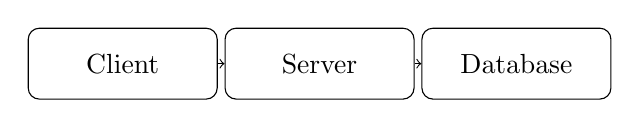
\begin{tikzpicture}[node distance=2.5cm, every node/.style={draw, rounded corners, minimum width=2.4cm, minimum height=0.9cm}]
    \node (client) {Client};
    \node (server) [right of=client] {Server};
    \node (db) [right of=server] {Database};
    \draw[->] (client) -- (server);
    \draw[->] (server) -- (db);
  \end{tikzpicture}
  \caption{Kiến trúc tổng quan}
  \label{fig:architecture}
\end{figure}
Xem Hình~\ref{fig:architecture}.

\subsubsection{Các thành phần}
\begin{table}[H]
  \centering
  \caption{Các thành phần của hệ thống}
  \label{tab:components}
  \begin{tabular}{lll}
    \toprule
    \textbf{Thành phần} & \textbf{Công nghệ} & \textbf{Vai trò} \\
    \midrule
    Client & Web & Giao diện người dùng \\
    Server & REST API & Xử lý nghiệp vụ \\
    Database & SQL & Lưu trữ dữ liệu \\
    \bottomrule
  \end{tabular}
\end{table}

\subsection{Thiết kế cơ sở dữ liệu}
